
\documentclass[english]{article}
\usepackage[utf8]{inputenc}
\usepackage[margin=1in]{geometry}
\usepackage{graphicx,wrapfig,lipsum}
\usepackage{caption}
\usepackage{refstyle}
\usepackage{titlepic}
\usepackage{graphicx}
\usepackage{grffile}
\usepackage{babel}
\usepackage{parskip}
\textwidth = 426pt
\oddsidemargin = 17pt


\title{Cos301 : User Manual\\
	for the SmartCard Application\\
	}
\date{\today}
\graphicspath{{Pictures/}}

\begin{document}
	\maketitle
	\begin{figure}[!t]
		
\includegraphics{up_logo.png}
	\end{figure}
	\begin{minipage}{0.4\textwidth}
		\begin{flushleft} \large
			\textbf{NAMES:}\\[0.4cm]
			Mufamadi {Khodani} \\
			Setoaba {Phuti} \\
			Dandashe {Kagiso Xolo} \\
			Mashaba {Mpho} \\
			Mathe {Musa} \\
			Ntsoane {Thabo}\\
		\end{flushleft}
	\end{minipage}
	\begin{minipage}{0.4\textwidth}
		\begin{flushright} \large
			\textbf{STUDENT NUMBER:} \\[0.4cm]
			u14197520 \\
			u13032616 \\
			u14245681 \\
			u14309999 \\
			u15048030 \\
			u15107532 \\
		\end{flushright}
\end{minipage}

	
	\pagenumbering{gobble}
	\newpage

	\tableofcontents
	

	\pagenumbering{arabic}
	
\newpage
	\section{System Overview}
	The SmartCard system is a mobile-based application that is used to transfer business data from one device to another using either NFC or QR-Code scanner.The application should be free to download from either a mobile phone application store or similar services. 
	
	\section{System Configuration}
	The SmartCard system operates on mobile devices with Android operating system. It is compatible with
	Android 4,1 (jelly bean) API 16 and higher versions. The application requires connection to Internet in order to
	save data to database. A virtual business card will be generated for the user using the information the user signed up with and will then be transmitted with a single tap using the NFC too available on their smart device. Alternatively the smart device’s camera will be used to scan the QR code on another device. After
	installation on the device, SmartCard can be used immediately without any further configuration.
	\section{Installation}
	The most recent apk has been made available on our GIT reprository for installation on a device. 
	
	Download the apk from the website and install on your device. For specific instruction on how to install application on specific device refer to
	device’s manual.
	
	Alternatively the application should be available for download and install on google play store.
	

	\section {Using The System}
	\subsection{Getting started}
	Upon opening the system, the following mainscreen should be visible.
		
			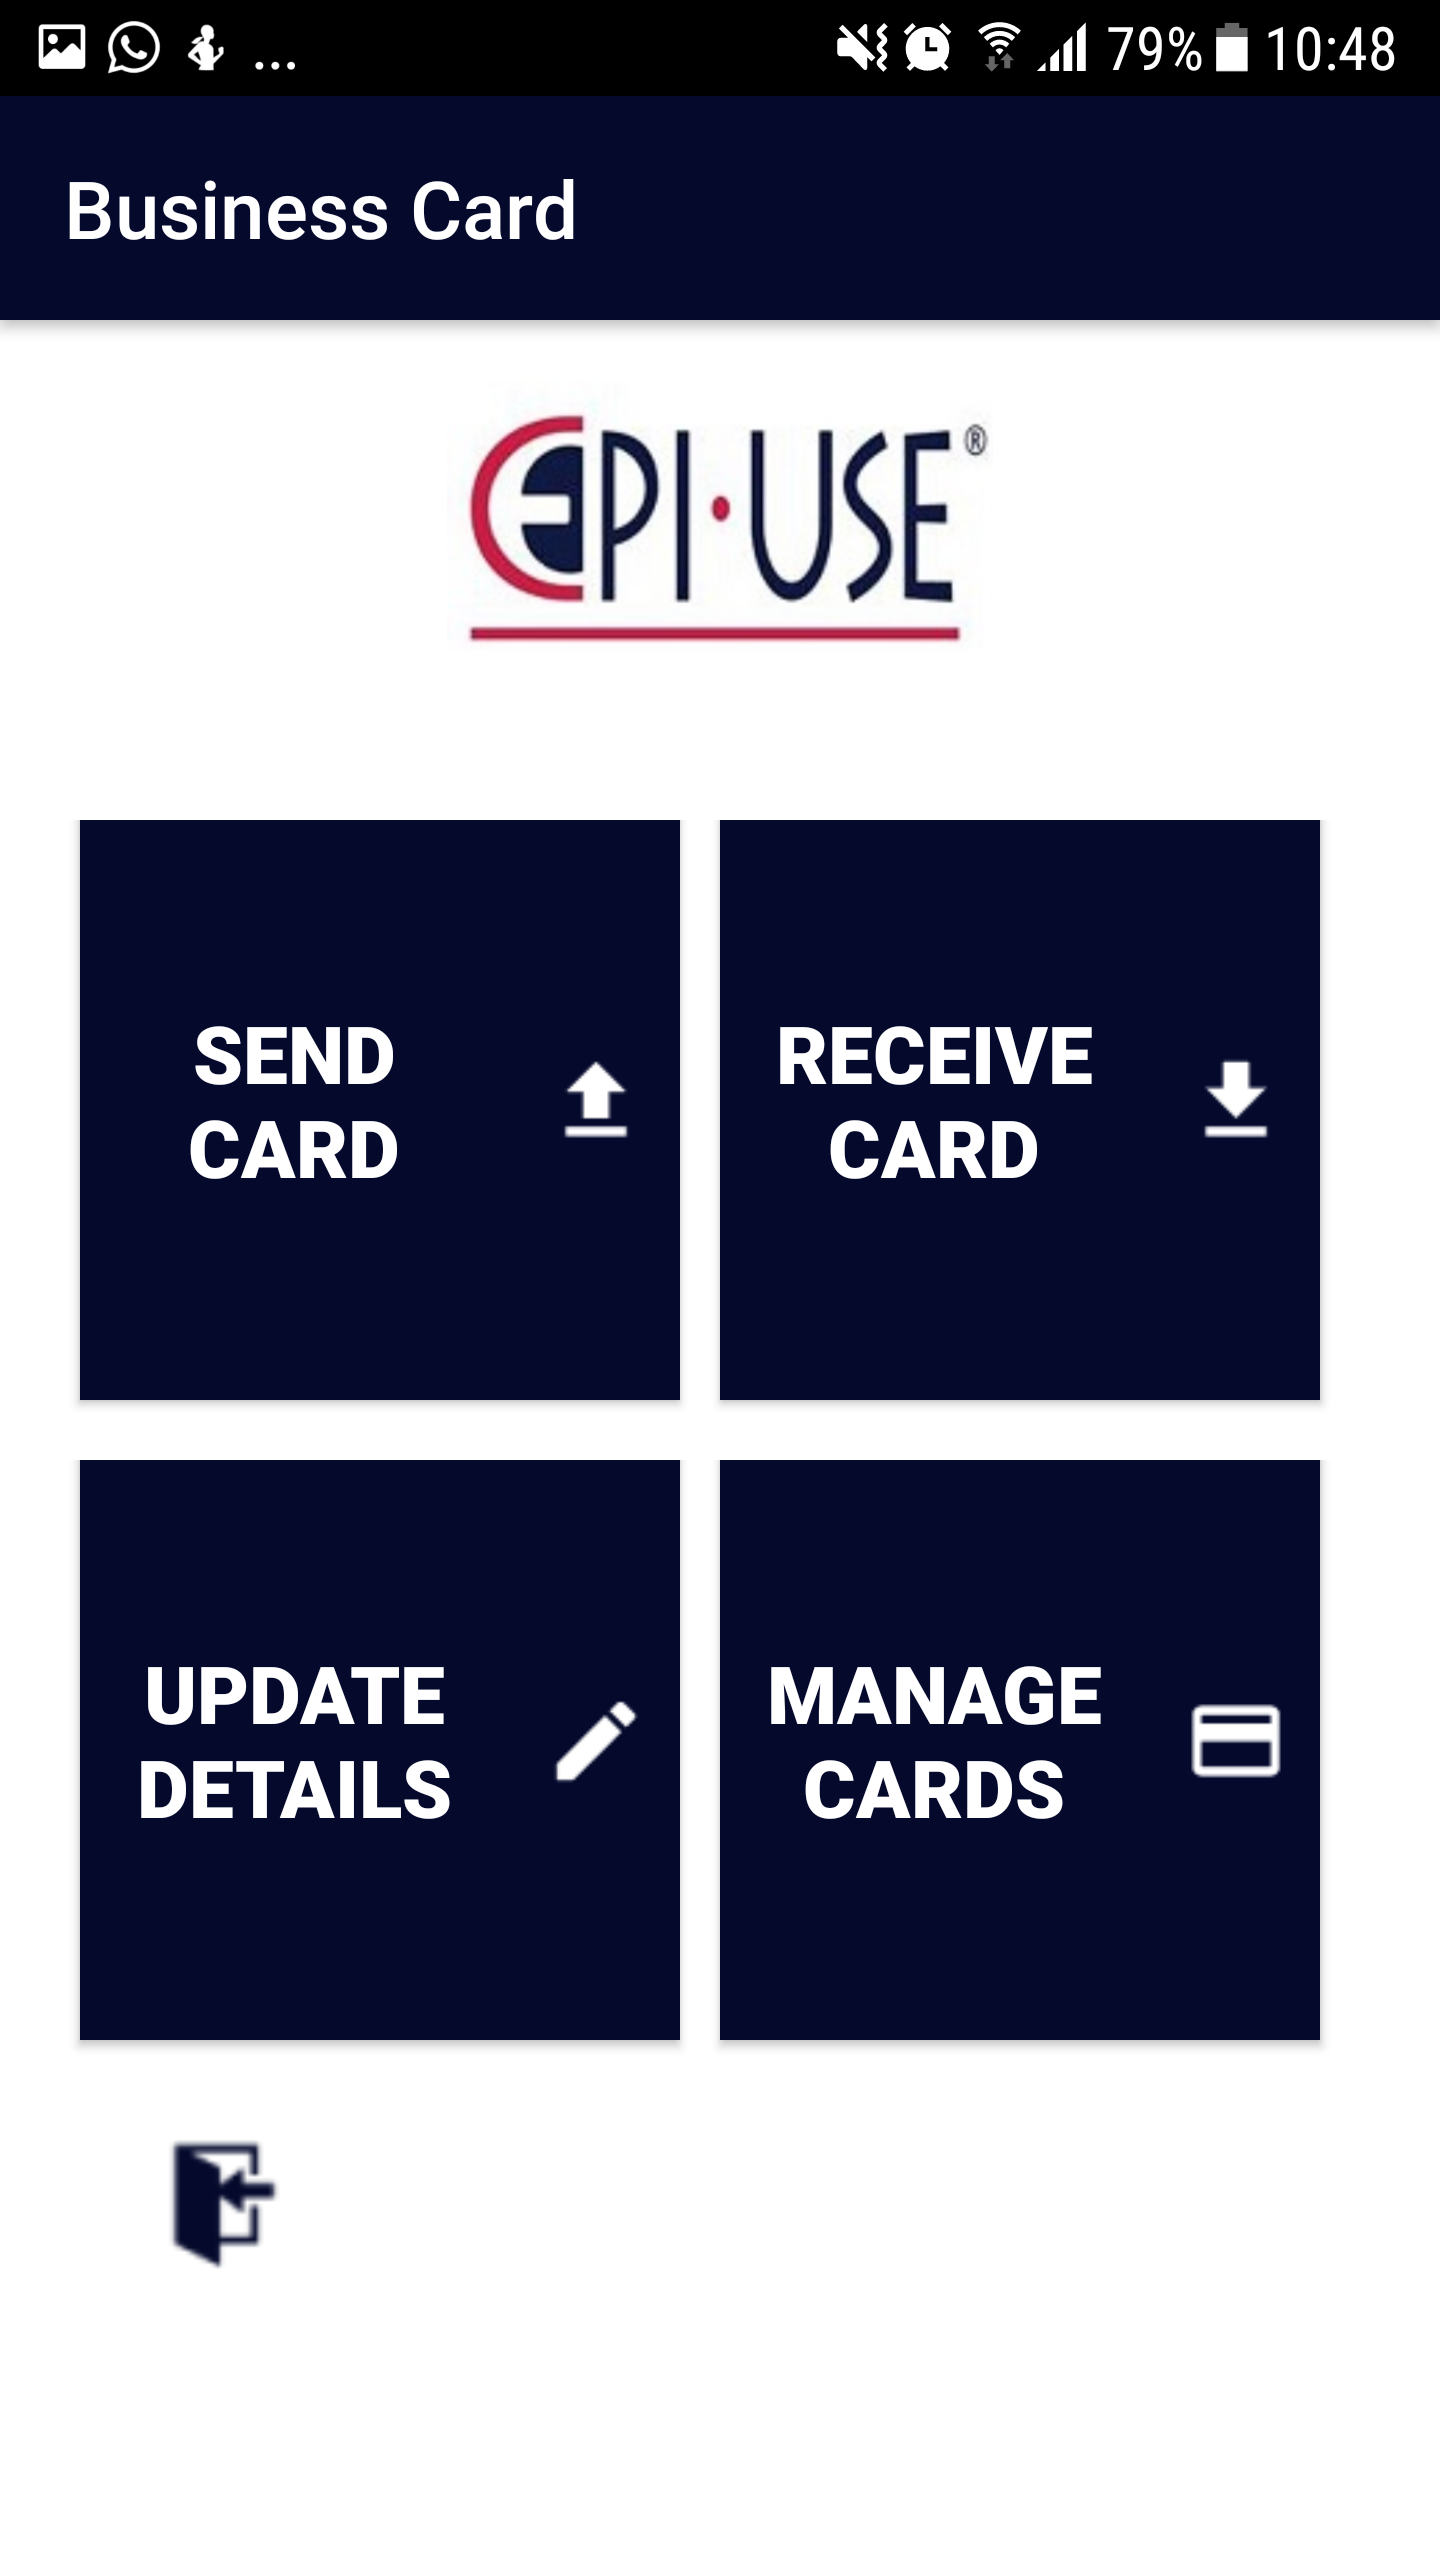
\includegraphics{Main.png}
	\begin{itemize}	
		\item How to sign up:
		
		
		\begin{enumerate}
			\item Upon opening the application, select emph{Register now}.
			\item Input your details on the provided form.
			

			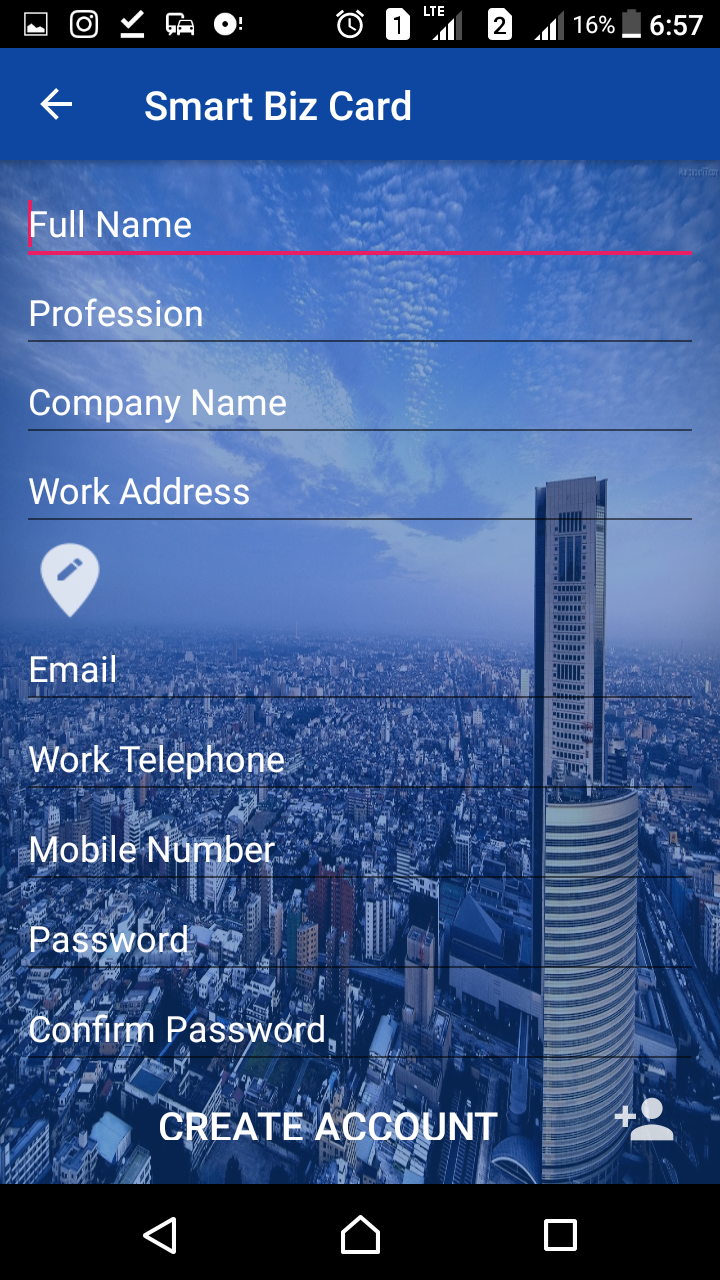
\includegraphics{Sign_up.png}
		
			\item Select emph{Create Account}.
			 
		\end{enumerate}

		\end{itemize}
		\begin{itemize}
		\item How to login:
		

			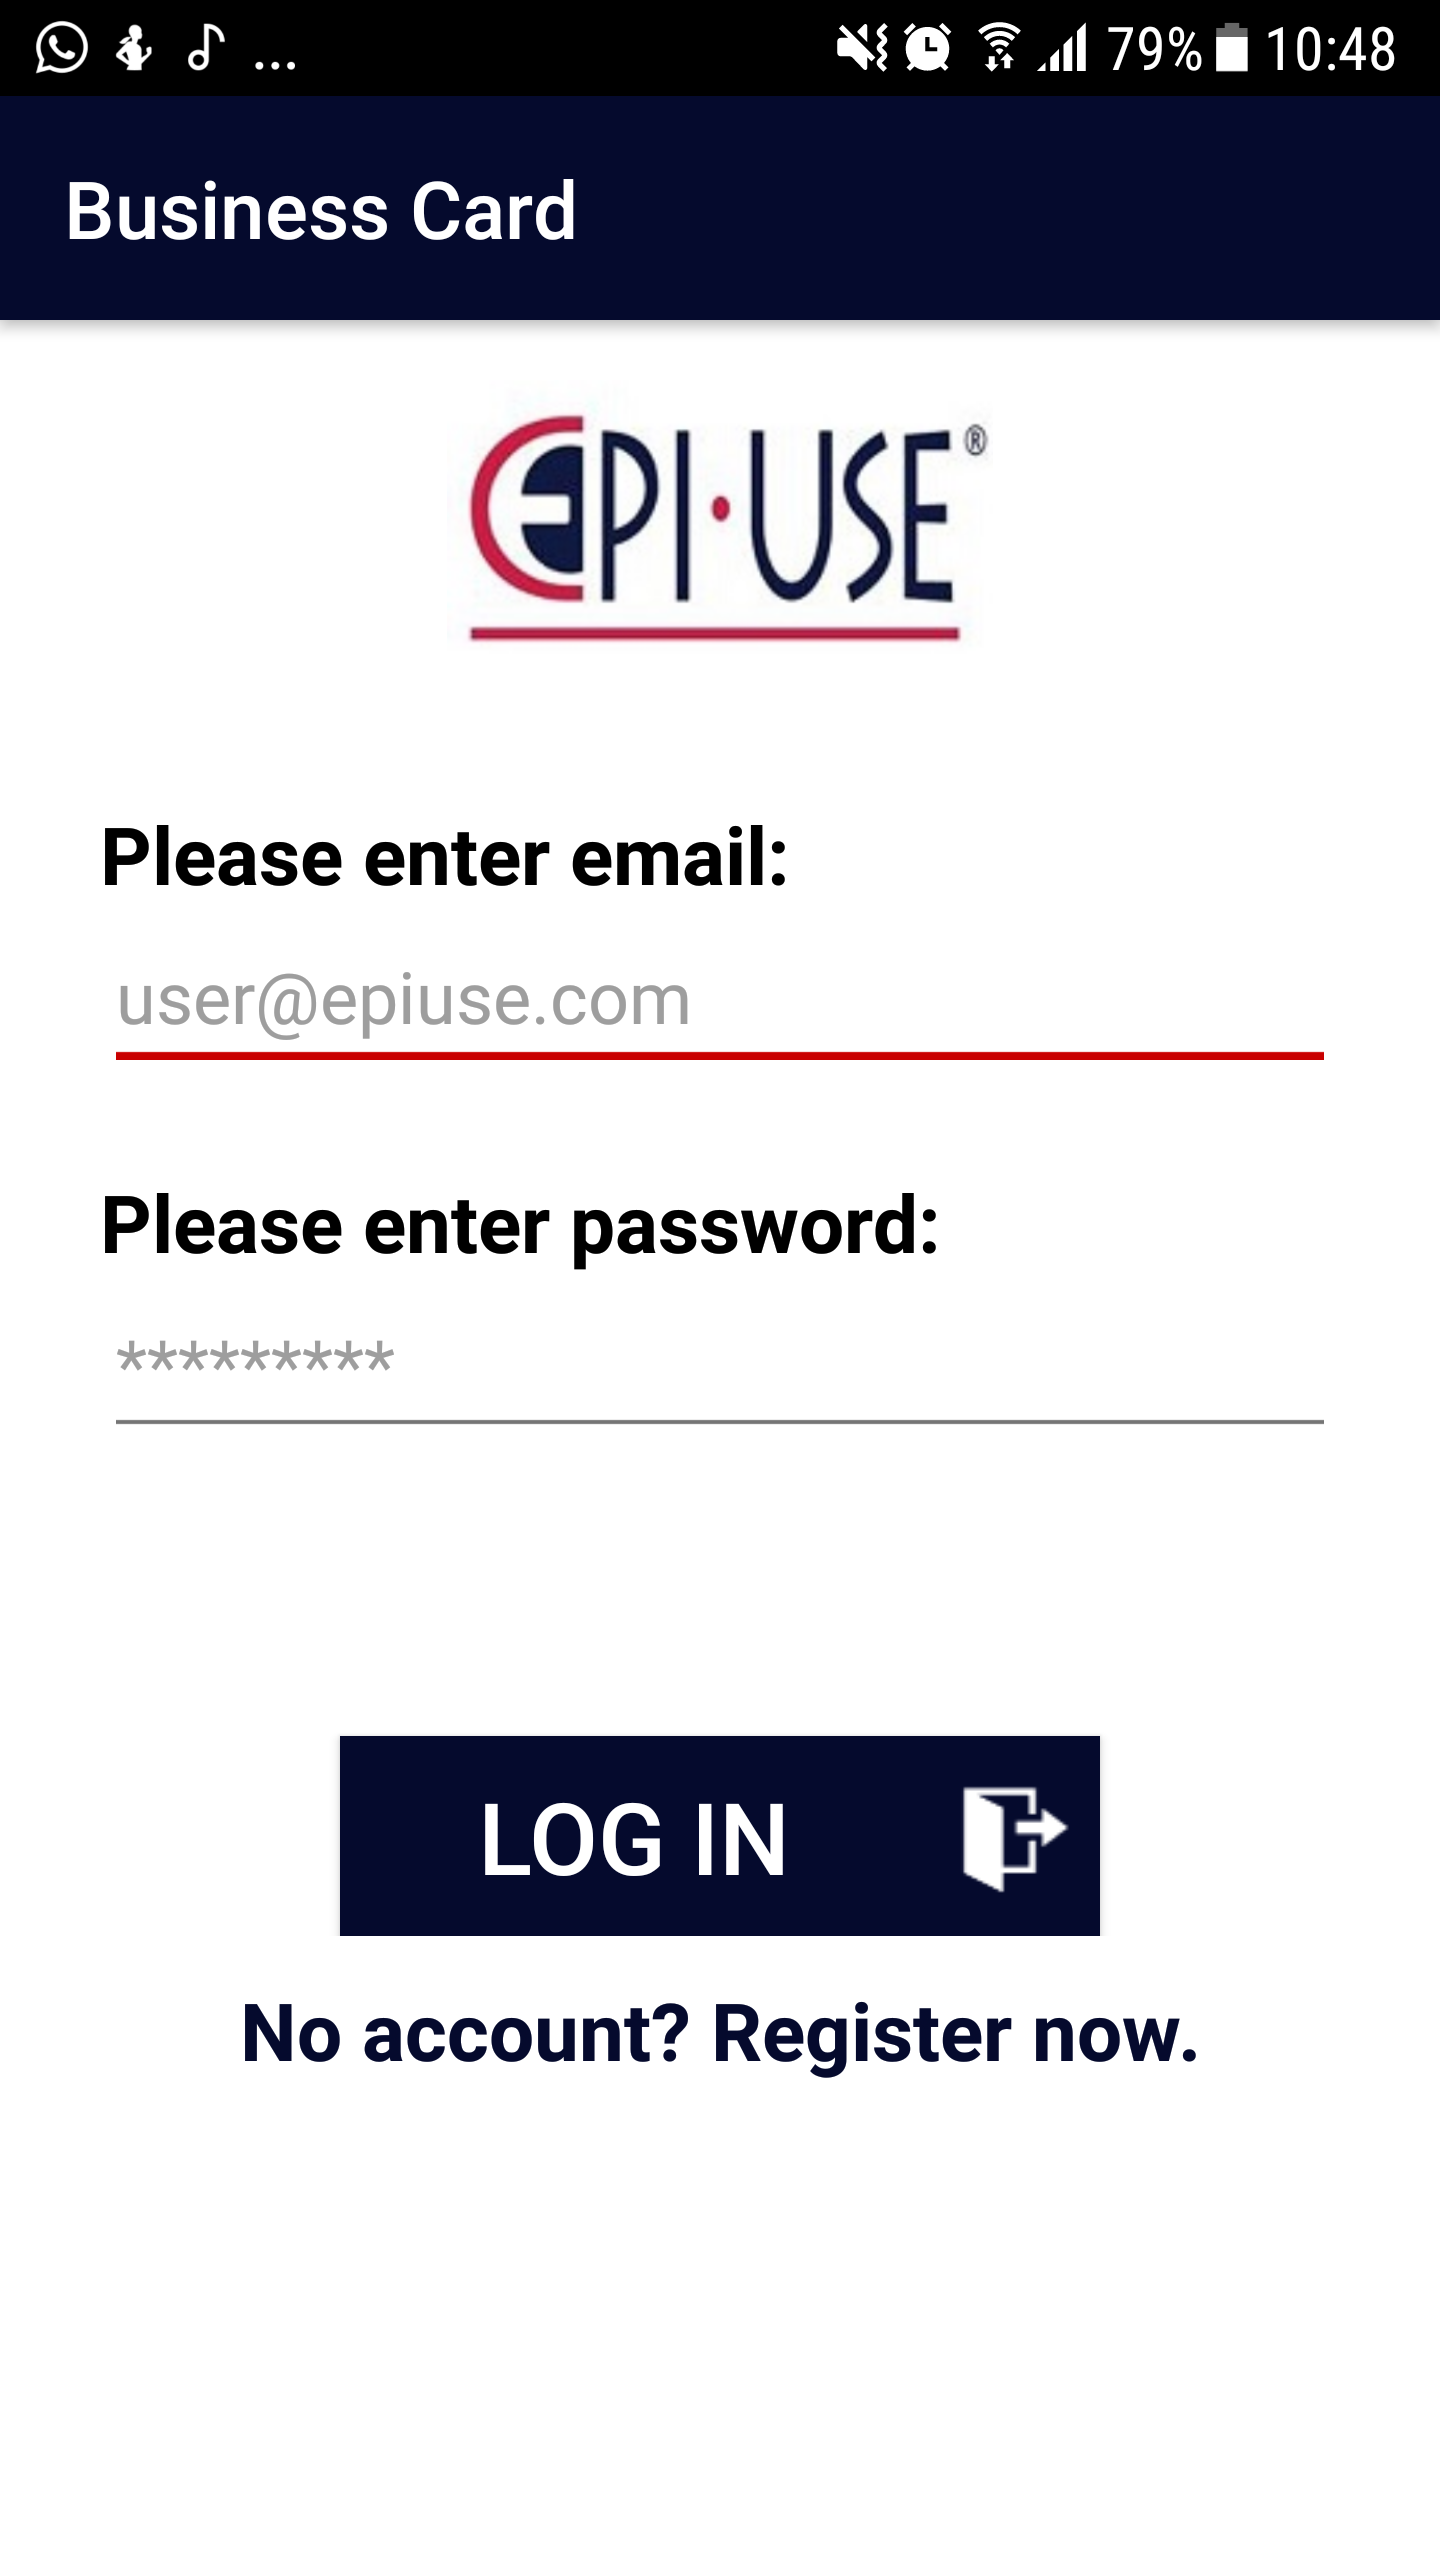
\includegraphics {Login.png}

		\end{itemize}
		\subsection{Sending business card}
		\begin{itemize}
		\item Sending through NFC:
		\begin{enumerate}
			\item From the main screen select emph{SEND CARD}
			\item Select emph{NFC}
			\item Simultaneously tap the screen and touch the phone with another device.
		\end{enumerate}
		\item Sending through QR code:
		\begin{enumerate}
			\item From the main screen select emph{SEND CARD}.
			\item Select emph{QR CODE}.
			\item Select emph{GENERATE CODE}.
			\item Allow another device to scan the code that was generated using their camera.
		\end{enumerate}
	\end{itemize}

\subsection{Recieving business card}
	\begin{itemize}
		\item Recieving through NFC
		\begin{enumerate}
			\item From the main screen select emph{SEND CARD}
			\item Select emph{NFC}
			\item Simultaneously tap the screen and touch the phone with another device.
		\end{enumerate}
		\item Recieving through scanning QR Code
		\begin{enumerate}
			\item From the main screen select emph{SEND CARD}.
			\item Select emph{QR CODE}.
			\item Select emph{SCAN CODE}.
			\item Scan the QR Code on another device to capture the data.
		\end{enumerate}
	\end{itemize}
	
	\section {Troubleshooting}
		In case of failure to send or recieve you will recieve a pop up notification to let you know that the operation has failed and you will either have to try again or cancel the opration.
	
\end{document}
